\chapter{Resampling to ATLAS and CMS Geometries}\label{sec:resampling}

In addition to the results presented so far, we show in this section how the end-to-end reconstruction would perform on calorimeters with granularity and geometry similar to those of the ATLAS and CMS calorimeters. Since the REC dataset (see Section~\ref{sec:data}) is generated using the geometry of the proposed LCD detector, it has a much higher granularity than the current-generation ATLAS and CMS detectors. To visualize how our calorimeter data would look with a coarser detector, we linearly extrapolate the contents of each event to a different calorimeter geometry, using a process we have termed "resampling". To keep the resampling procedure simple, we discard the HCAL information and consider only the ECAL 3D array.

\begin{table*}[tbp]
\centering
\caption{Detailed description of the three detector geometries used in this study: the baseline CLIC ECAL~\cite{CLIC_geometry} and the ATLAS~\cite{Aad:2008zzm} and CMS~\cite{Chatrchyan:2008aa} ECALs.\label{tab:resampling_geometry}}
\begin{tabular}{c|c|ccc|c}
\hline
\multirow{2}{*}{Parameter} & \multirow{2}{*}{\textbf{CLIC}} & \multicolumn{3}{c|}{\textbf{ATLAS}} & \multirow{2}{*}{\textbf{CMS}} \\
            &               & 1st layer & 2nd layer & 3rd layer & \\
\hline
$\Delta \eta$         & 0.003  & 0.025 /8 & 0.025 & 0.5   & 0.0175 \\
$\Delta \phi$         & 0.003  & 0.1      & 0.025 & 0.025 & 0.0175 \\
Radiation Length [cm] & 0.3504 & 14       & 14    & 14    & 0.8903 \\
Moliere radios [cm]   & 0.9327 & 9.043    & 9.043 & 9.043 & 1.959  \\
\hline 
\end{tabular}
\end{table*}

A not-to-scale example of the full procedure is shown in Figure~\ref{fig:resampling}. In this example, we resample the input to a regular square grid with lower granularity than the input data. The operation is simplified in the figure, in order to make the explanation easy to visualize. The actual ATLAS and CMS calorimeter geometries are more complex than a regular array, as described in Table~\ref{tab:resampling_geometry}.

In the resampling process, we first extrapolate each energy value from the grid of CLIC cells to a different geometry. To do so, we scale the content of each CLIC cell to the fraction of overlap area between the CLIC cell and the cell of the target geometry. When computing the overlap fraction, we take into account the fact that different materials have different properties (Moliere radius, interaction length, and radiation length). For instance, CLIC is more fine-grained than CMS or ATLAS detectors, but the Moliere radius of the CLIC ECAL is much smaller than in either of those detectors. This difference determines an offset in the fine binning. Thus, when applying our resampling procedure we normalize the cell size by the detector properties. The Moliere radius is used for $x$ and $y$ re-binning, and radiation length is used for the $z$ direction. At this point we have a good approximation for how the event would look in a calorimeter with the target geometry.

To complete the resampling process, we invert the procedure to go back to our original high-granularity geometry. This last step allows us to keep using the model architectures that we have already optimized. It adds no additional information that would not be present in the low-granularity geometry. This up-sampling also allows us to deal with the irregular geometry of the ATLAS calorimeter by turning it into a neat grid. With no up-sampling, it would not be possible to apply the CNN and GN models. This procedure was validated by comparing total energies before and after resampling, and by visually comparing resampled grids. The energy matches for events were not exact, due to losses at the edge of the resampling grid, and the shower resolutions became much less granular after resampling, but overall the energies and distributions matched before and after the procedure was applied.

\begin{figure}[htbp]
    \centering
    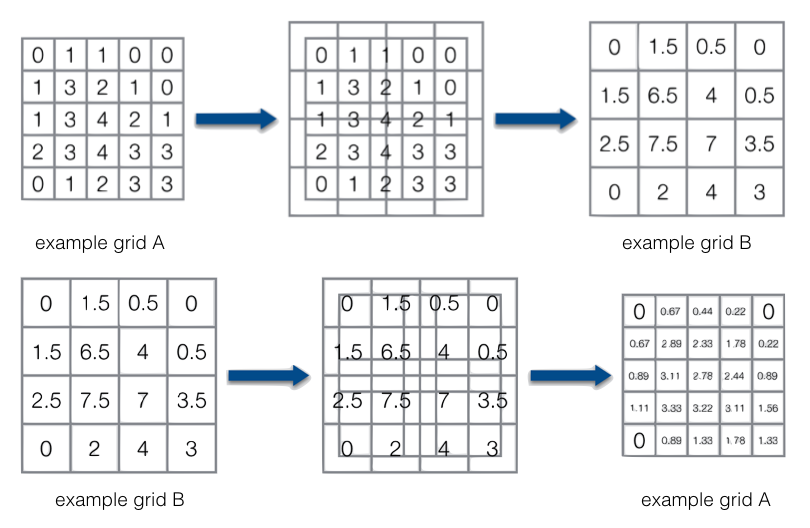
\includegraphics[scale=0.3, clip]{Images/Calo/resampling.png}
    \caption{Example of the resampling procedure used to emulate CLIC data on a different detector geometry (the example shown here is simply a larger grid). First, we extrapolate hit information from one geometry to another (top). Next, we extrapolate back to the original geometry (bottom). This allows us to emulate the rougher granularity of the second geometry, while keeping data array sizes constant and enabling us to use the models we have already developed for the CLIC dataset. Note that some information is lost at the edges.}
    \label{fig:resampling}
\end{figure}

%\begin{center}
%\begin{tabular}{ l | c c c c c }
% Detector & Cell Size ($\Delta\eta\times\Delta\phi$) & Image Size & Material & $\Chi_0$ [cm] & $R_M$ [cm] \\ 
%\hline
%CLIC          & $0.003\times0.003$     & $25\times25\times25$ & tungsten & 0.35 & 0.92       \\
%CMS           & $0.0175\times0.0175$   & $5\times5\times1$    & lead tungstate & 0.89 & 1.96 \\  
%ATLAS layer 1 & $0.003\times0.1$       & & & & \\
%\caption{Calorimeter properties for the three detector geometries considered. UPDATE FORMAT TO FIT IN ONE COLUMN AND ADD ATLAS 3 LAYERS}
%\end{tabular}
%\end{center}

The resampling procedure comes with a substantial simplification of the underlying physics process. First of all, the information at the edge of the grid is imperfectly translated during the resampling process, leading to worse performance than what could theoretically be achieved in the actual CMS and ATLAS detectors. Also, this simple geometrical rescaling doesn't capture many other detector characteristics. For example, the CMS ECAL detector has no depth information, but being homogeneous it provides a very precise energy measurement. Our resampling method only captures geometric effects, and would not be able to model the improvement in energy resolution. Furthermore, we are unable to include second-order effects such as gaps in the detector geometries. Despite these limitations, one can still extract useful information from the resampled datasets, comparing the classification and regression performances of the end-to-end models defined in Sections~\ref{sec:classification} and~\ref{sec:regression} on different detector geometries.

Comparisons of classification ROC curves between network architectures and our BDT baseline are shown in Figure~\ref{fig:class_ROC_ATLAS_CMS} for ATLAS-like and CMS-like geometries. Here we can see that the previously observed performance ranking still holds true. The GN
model performs best, followed by the CNN, then the DNN. All three networks outperform the BDT baseline. The effect is less pronounced after the CMS-like resampling, due to the low granularity and the single detector layer in the z direction.

\begin{figure}[htbp]
    \centering
    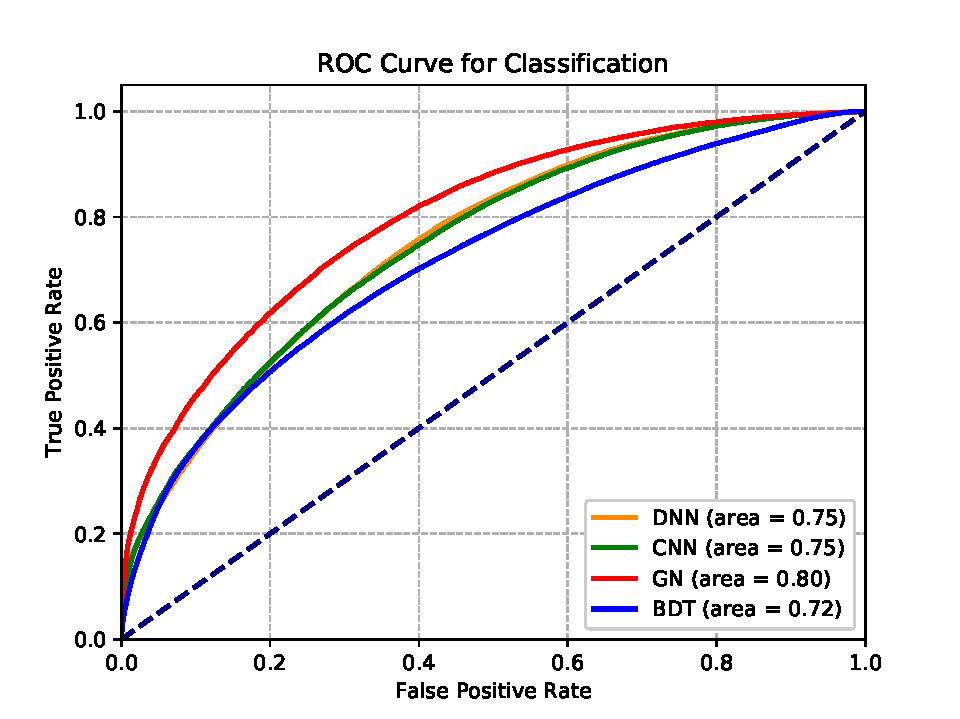
\includegraphics[scale=0.5, clip]{Images/Calo/classification_ROC_ATLAS.pdf}
    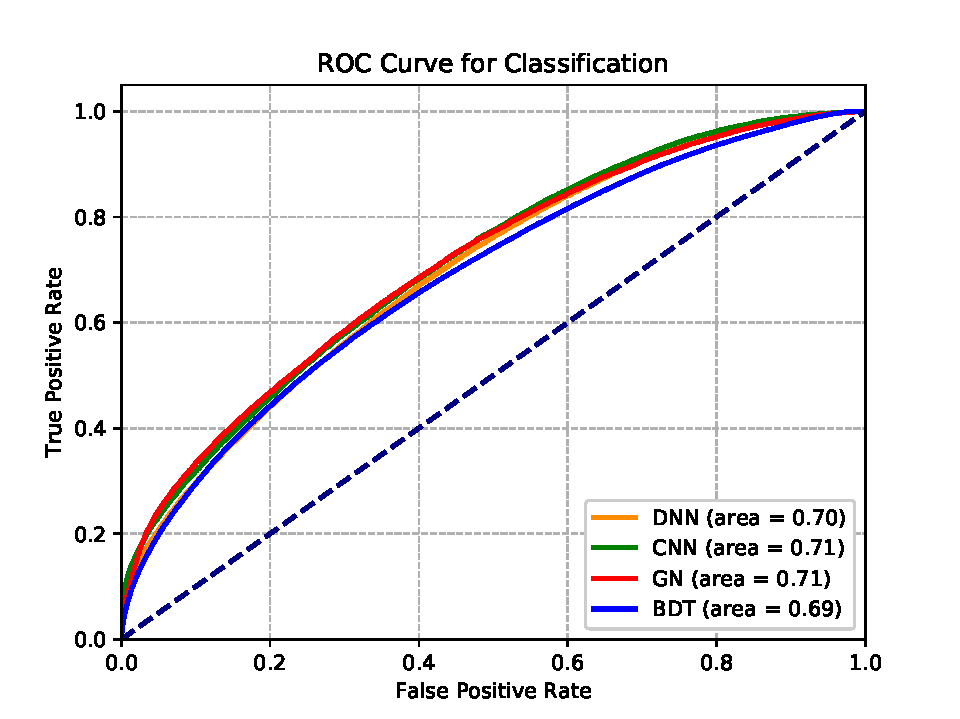
\includegraphics[scale=0.5, clip]{Images/Calo/classification_ROC_CMS.pdf}
    \caption{ROC curve comparisons for variable-angle $\gamma$/$\pi^0$ classification on data resampled to ATLAS-like (top) and CMS-like (bottom) geometries. Algorithms compared are DNN, CNN, GoogLeNet (GN), and BDT.}
    \label{fig:class_ROC_ATLAS_CMS}
\end{figure}

Regression results are shown in Figure~\ref{fig:reg_resampled_gamma_ATLAS_CMS} and~\ref{fig:reg_resampled_pi0_ATLAS_CMS}, for photons and neutral pions (we did not train electrons or charged pions for this comparison). Here we have included the regression baselines, DNN networks, and CNN networks, but not GN (which we did not train on resampled data). The results obtained for the ATLAS-like resampling match those on the REC dataset, with DNN and CNN matching the BDT outcome in terms of bias and surpassing it in resolution. With the CMS-like resampling the neural networks match but do not improves over the BDT energy regression resolution. Once again, this is due to the low spatial resolution in the CMS-like geometry, especially due to the lack of $z$ segmentation. We are unable to model the improved energy resolution from the actual CMS detector, so these energy regression results are based on geometry only.

\begin{figure*}[htbp]
\centering
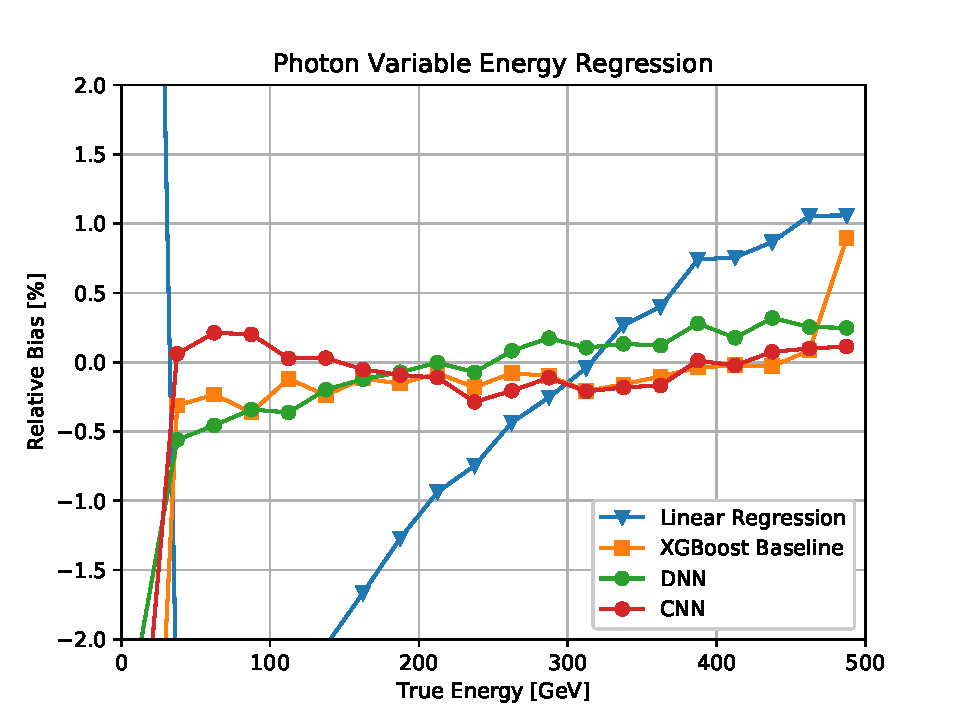
\includegraphics[width=0.38\textwidth]{Images/Calo/bias_vs_E_Gamma_variable_ATLAS.pdf}
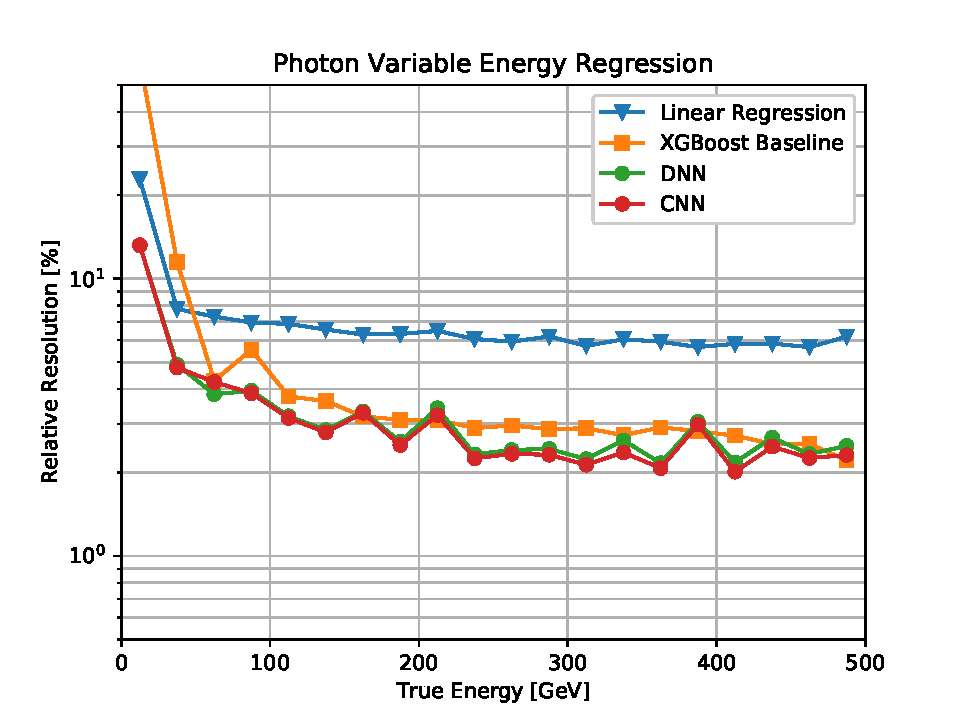
\includegraphics[width=0.38\textwidth]{Images/Calo/res_vs_E_Gamma_variable_ATLAS.pdf} \\
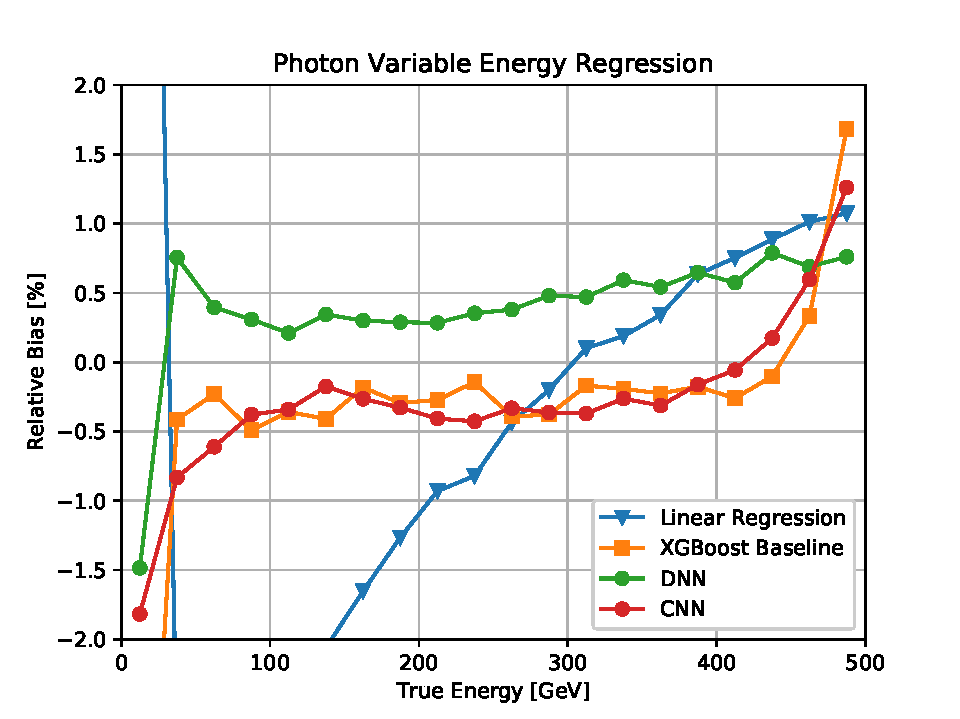
\includegraphics[width=0.38\textwidth]{Images/Calo/bias_vs_E_Gamma_variable_CMS.pdf}
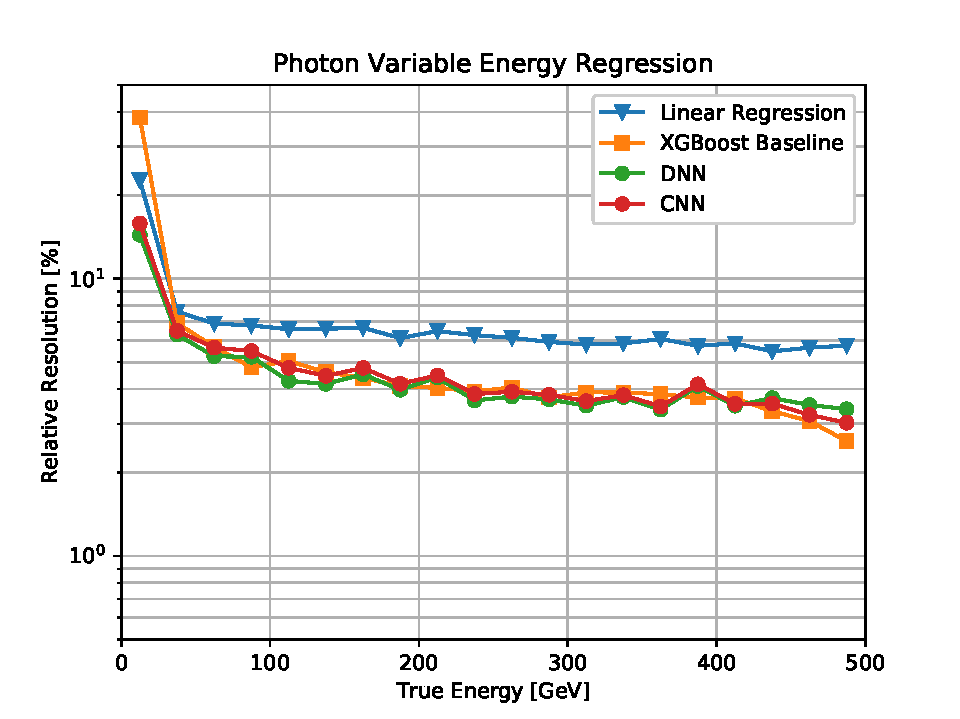
\includegraphics[width=0.38\textwidth]{Images/Calo/res_vs_E_Gamma_variable_CMS.pdf}
\caption{Bias (left) and resolution (right) as a function of true energy for energy predictions for photons, on variable-angle samples resampled to ATLAS-like (top) and CMS-like (bottom) geometries. \label{fig:reg_resampled_gamma_ATLAS_CMS}}
\end{figure*}

\begin{figure*}[htbp]
\centering
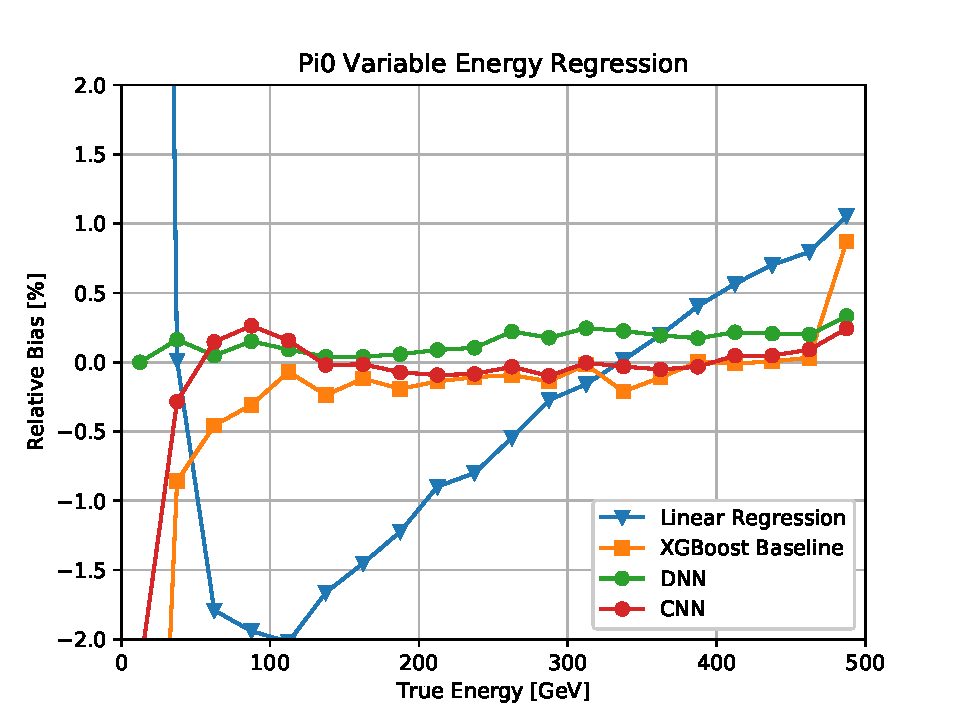
\includegraphics[width=0.38\textwidth]{Images/Calo/bias_vs_E_Pi0_variable_ATLAS.pdf}
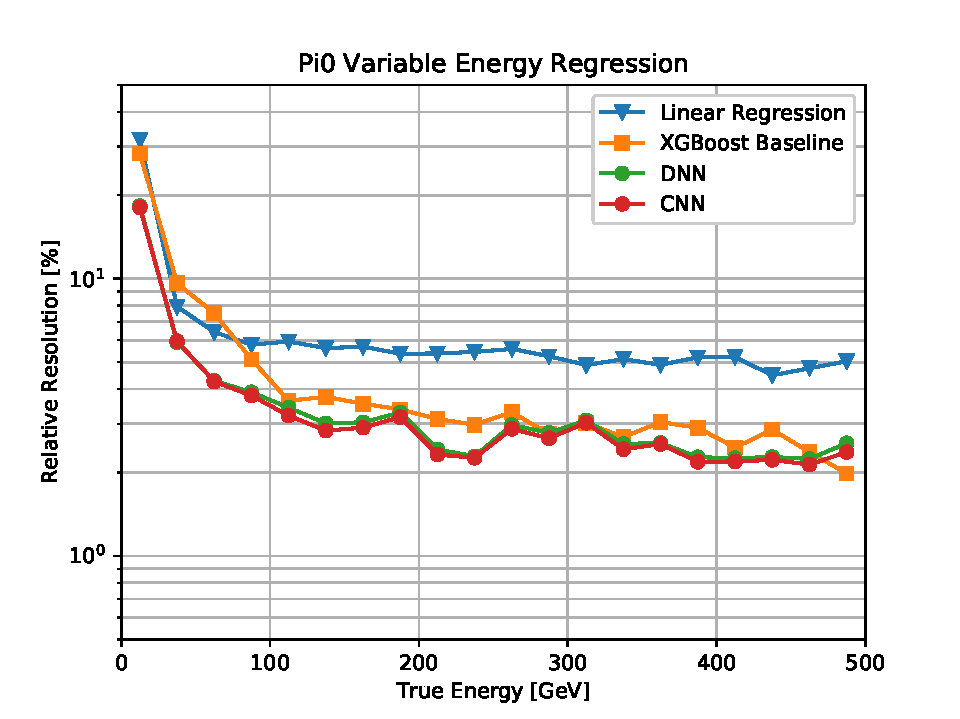
\includegraphics[width=0.38\textwidth]{Images/Calo/res_vs_E_Pi0_variable_ATLAS.pdf} \\
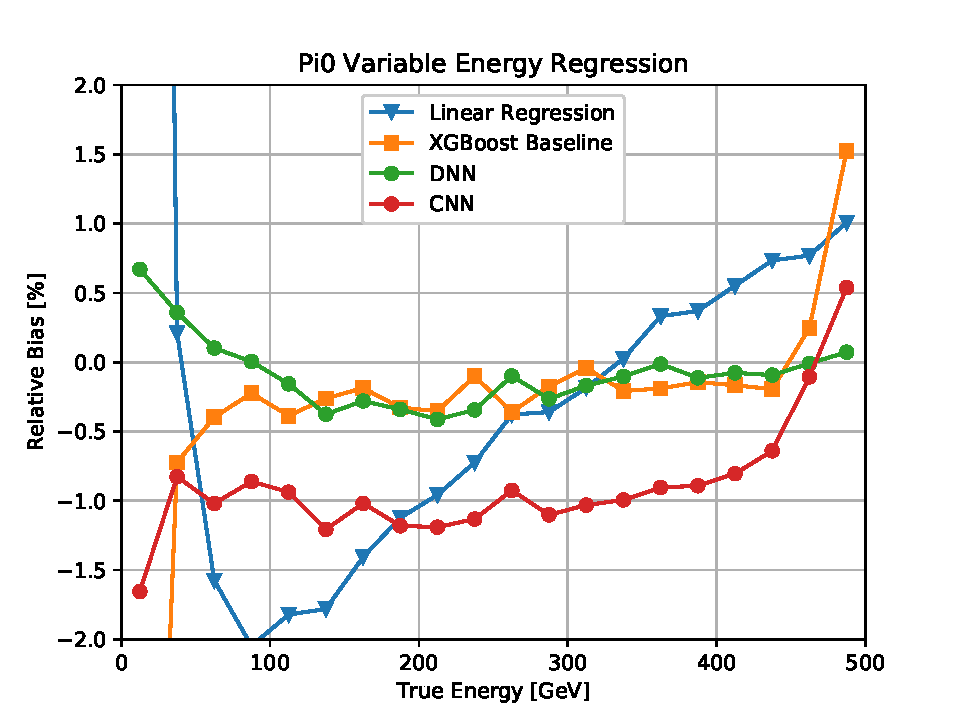
\includegraphics[width=0.38\textwidth]{Images/Calo/bias_vs_E_Pi0_variable_CMS.pdf}
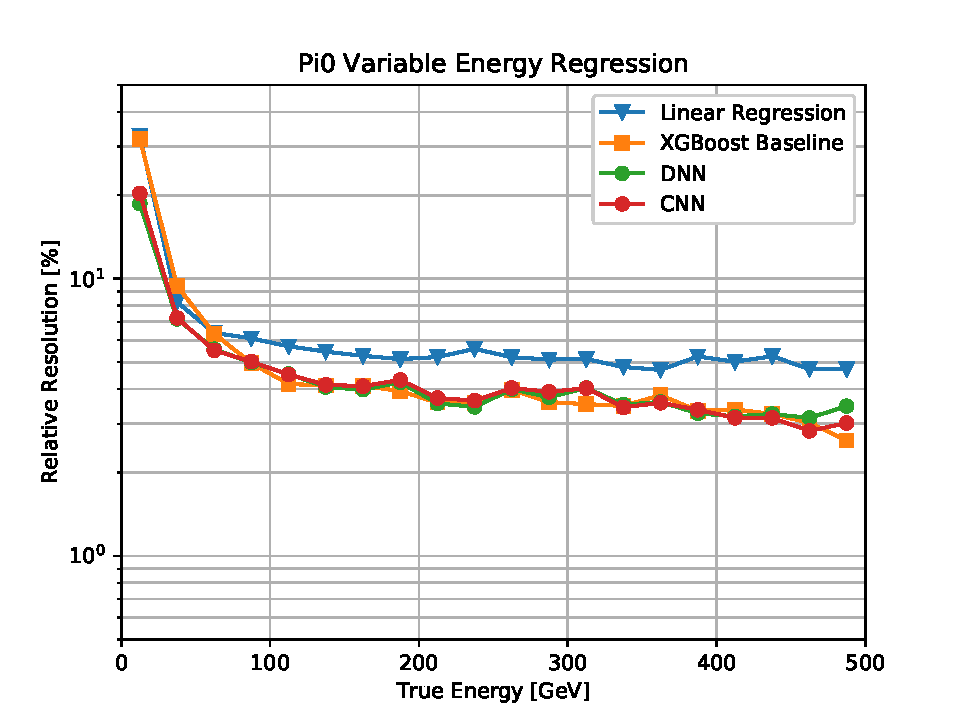
\includegraphics[width=0.38\textwidth]{Images/Calo/res_vs_E_Pi0_variable_CMS.pdf}
\caption{Bias (left) and resolution (right) as a function of true energy for energy predictions for \pizero, on variable-angle samples resampled to  ATLAS-like (top) and CMS-like (bottom) geometries.\label{fig:reg_resampled_pi0_ATLAS_CMS}}
\end{figure*}

\section{Calorimeter Window Size}\label{calo_rec_window_size}

The optimal window size to store for ECAL and HCAL is an important issue, since this impacts not only sample storage size, but also training speed and the maximum batch sizes which we could feed to our GPUs. 

From examinations of our generated samples, we found that an ECAL window of 25x25x25 and an HCAL window of 11x11x60 looked reasonable. To test this hypothesis, we performed training using the samples and classification architectures described in our previous studies~\cite{NIPS}, but with different-sized input samples. The architecture was altered to accommodate larger windows simply by increasing the number of neurons on the input layer. Results trained using an ECAL window of size 25x25x25 and 51x51x25 are shown in Figure~\ref{fig:classification_window}. From the similarity of these curves, we have decided that an expanded ECAL window size does not contain much additional useful information, and is thus not necessary for our problems.

\begin{figure*}[htbp]
    \centering
    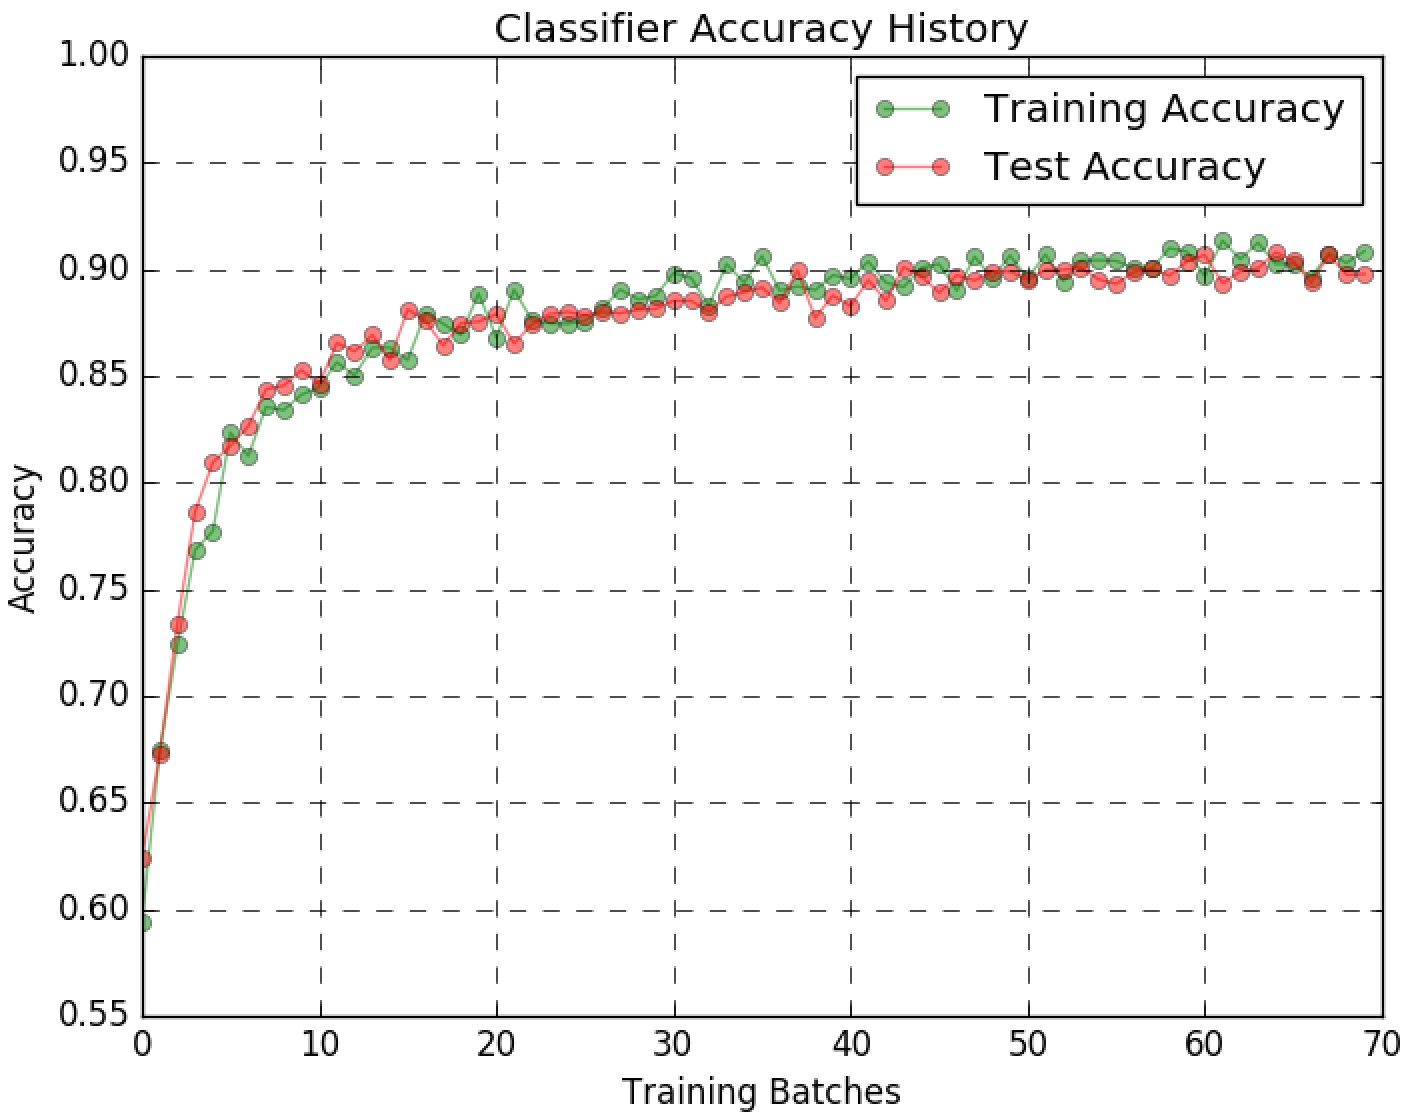
\includegraphics[width=0.45\textwidth]{Images/Calo/accuracy_small_window.png}
    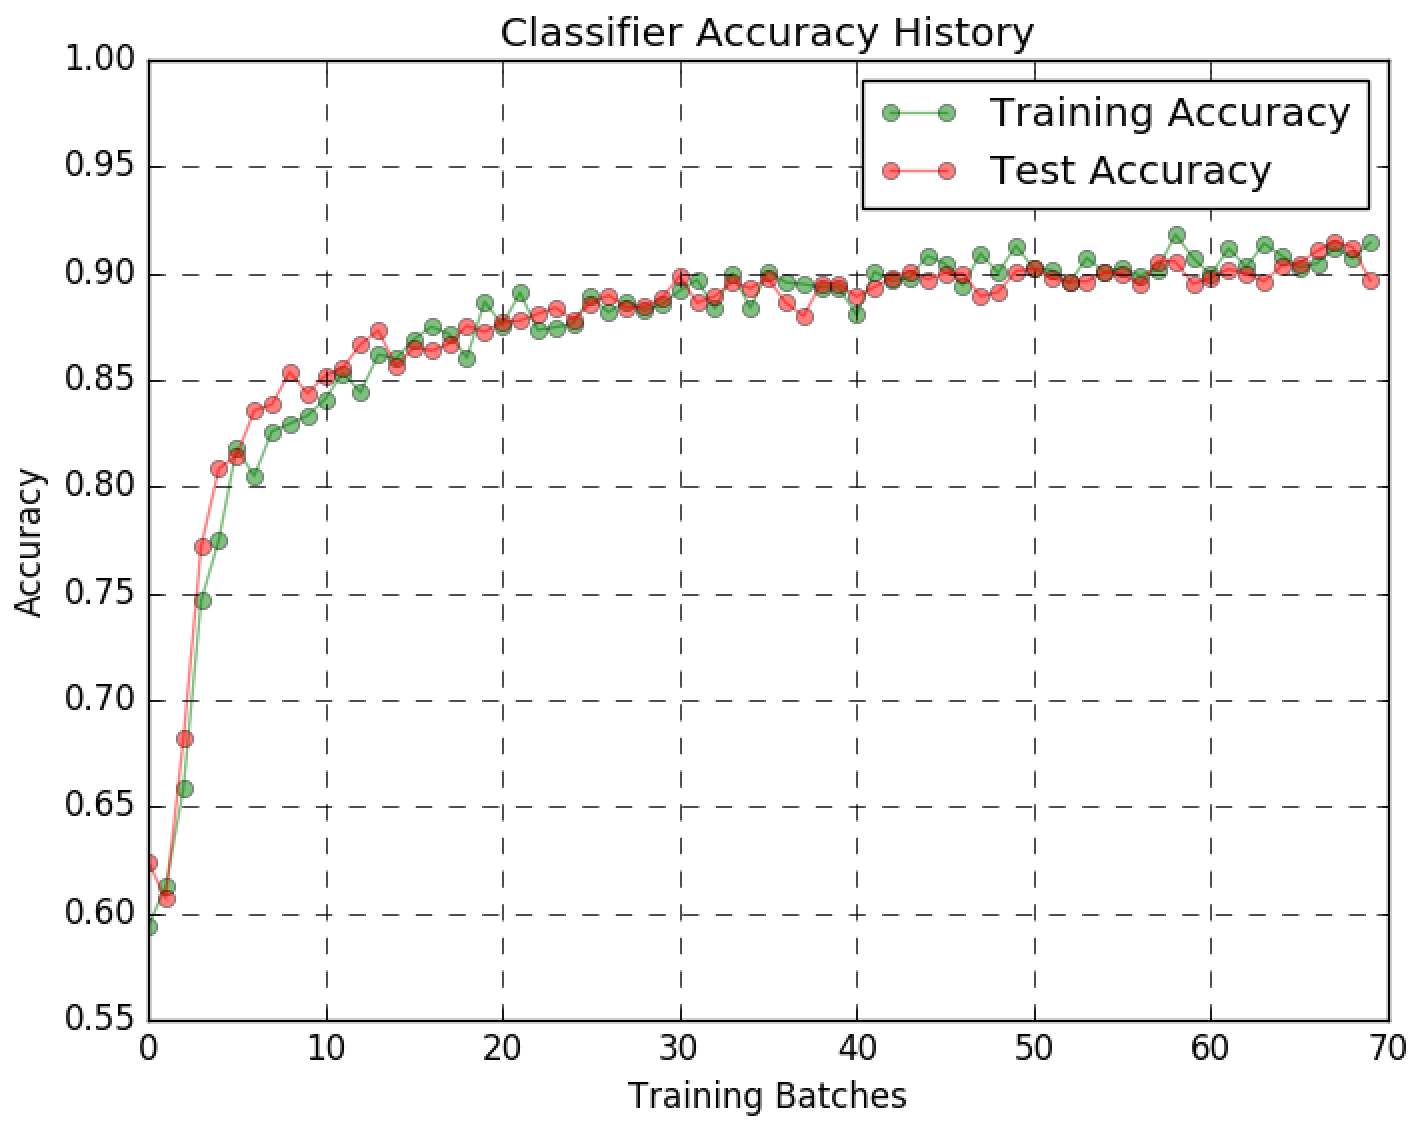
\includegraphics[width=0.45\textwidth]{Images/Calo/accuracy_large_window.png} \\
    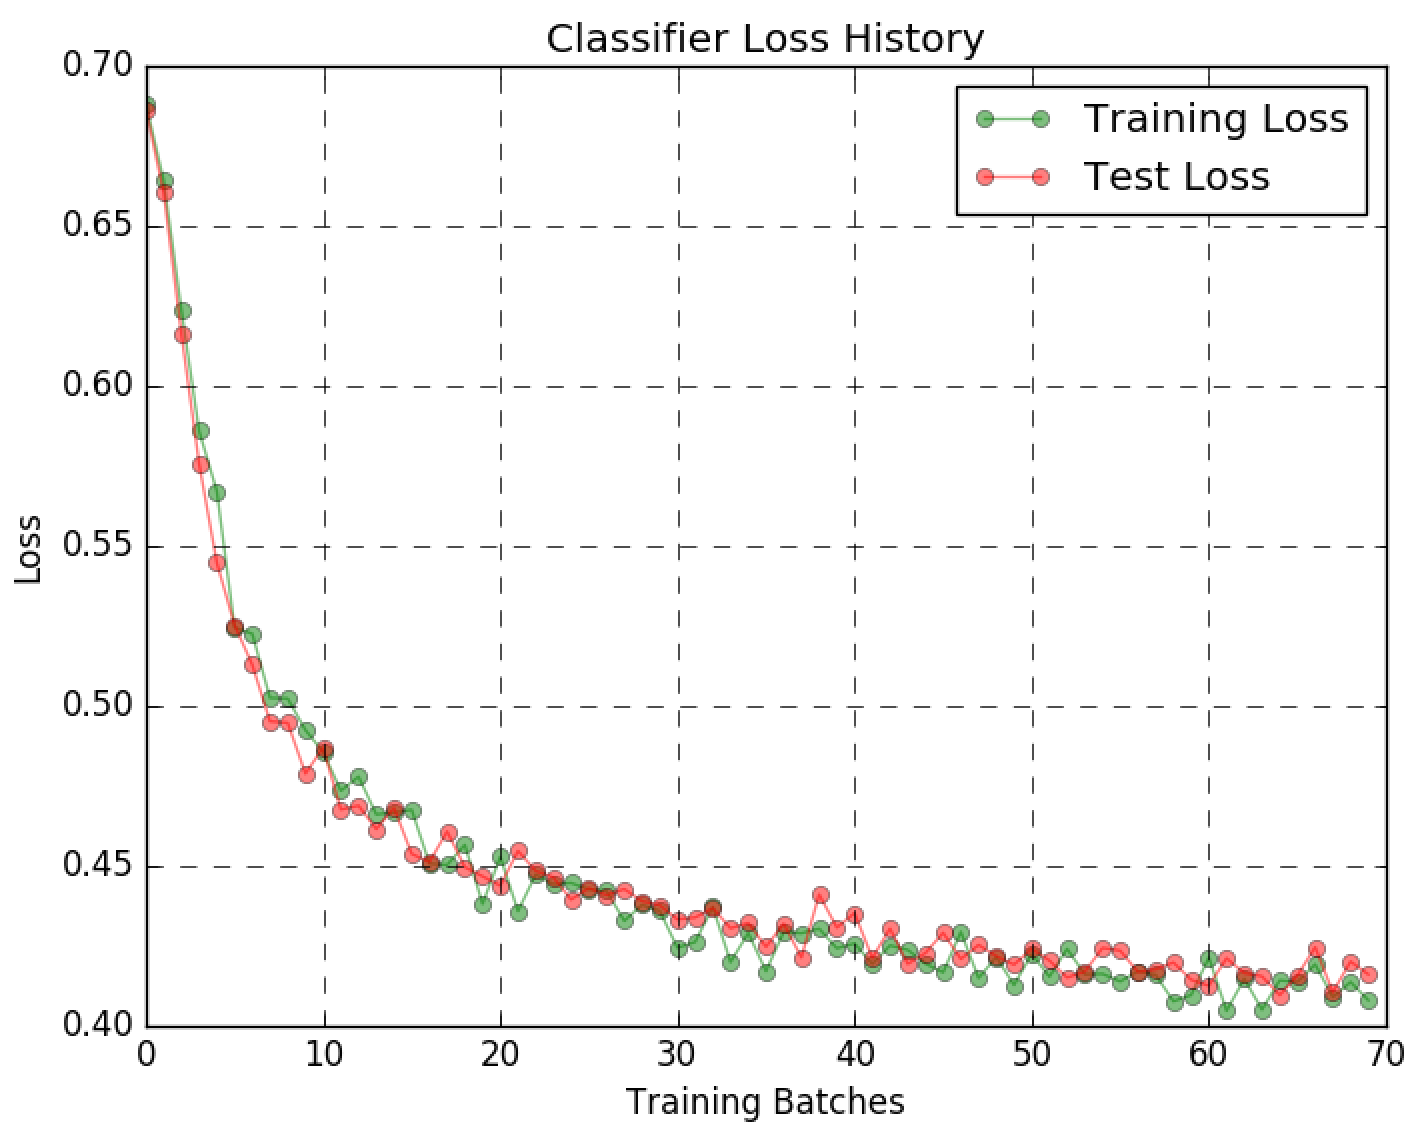
\includegraphics[width=0.45\textwidth]{Images/Calo/loss_small_window.png}
    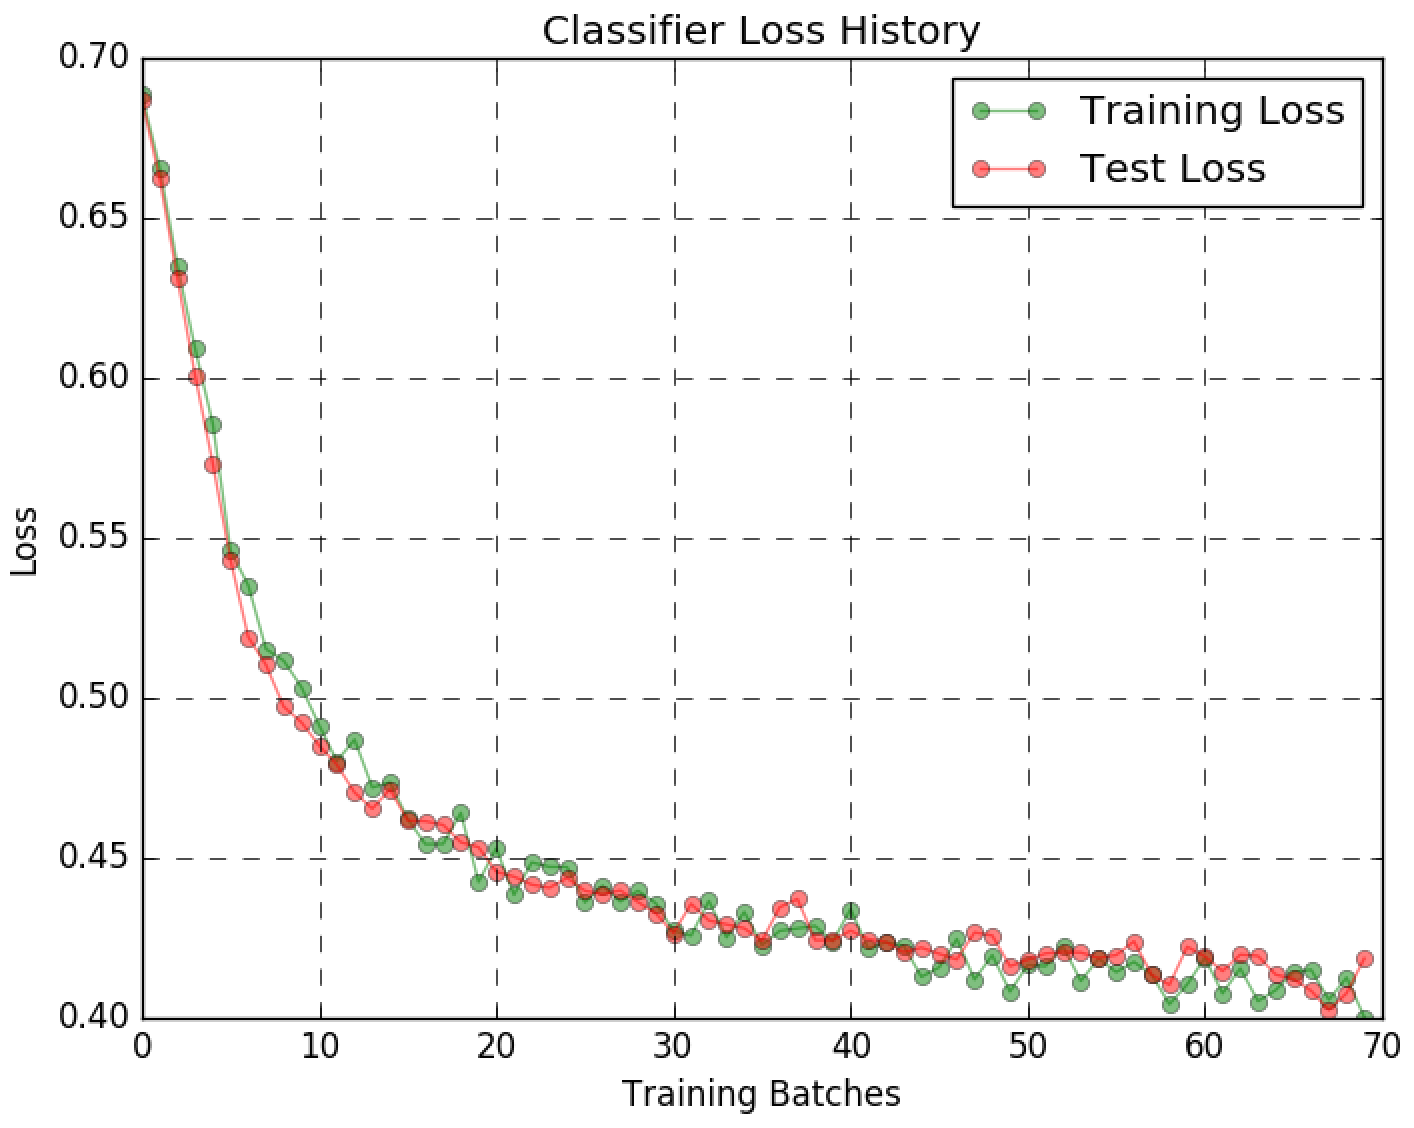
\includegraphics[width=0.45\textwidth]{Images/Calo/loss_large_window.png}
    \caption{Training history for different choices of the input 3D array zise: Accuracy (top) and loss (bottom) as a function of the training batch for photon/neutral pion classification, using a 25x25x25 (left) and 51x51x25 (right) ECAL window size.\label{fig:classification_window}}
\end{figure*}